\documentclass{article}

\usepackage[utf8]{inputenc}
\usepackage[margin=1.25in]{geometry}
\usepackage{amsmath, amssymb, amsthm}
\usepackage{graphicx}
\usepackage{mathdots}
\usepackage{esvect}
\setlength{\parskip}{1em}
\setlength{\parindent}{2em}
\usepackage{indentfirst}
\usepackage{matlab-prettifier}
\usepackage[T1]{fontenc}

\begin{document}

\begin{titlepage}
\centering
	\vspace*{\fill}
	{\huge\bfseries ROB521 A1 - PRM Maze Solver\par}
	\vspace{7cm}
	{\Large\itshape Ethan Rajah\par}
	{\Large February 28, 2025\par}
	\vspace*{\fill}
\end{titlepage}

\newpage
\section{Question 1}
The first question involves the implementation of a PRM algorithm to solve a maze.
The maze is represented as a 2D grid with obstacles and the goal is to construct a graph
of nodes and edges that connects the start and end points of the maze. The graph construction is limited
to a maximum of 500 samples and the number of edges per node is tuned as a hyperparameter.
The PRM algorithm is implemented by uniformly sampling 500 points in the maze,
filtering out points that are within 0.1 units of obstacles using the MinDist2Edges function,
and connecting each remaining point (now milestone) to its k-nearest neighbors. The k-nearest neighbors are found using
a squared distance metric and the edges are added only if they do not intersect with any obstacles
(found using the CheckCollision function). I found that k=8 was the optimal number of neighbors
to connect each node to for the 5x7 maze as it resulted in a good balance between computational efficiency
and high probability in generating a path. A sample graph is shown below in \textbf{Figure 1}.

\begin{figure}[h]
    \centering
    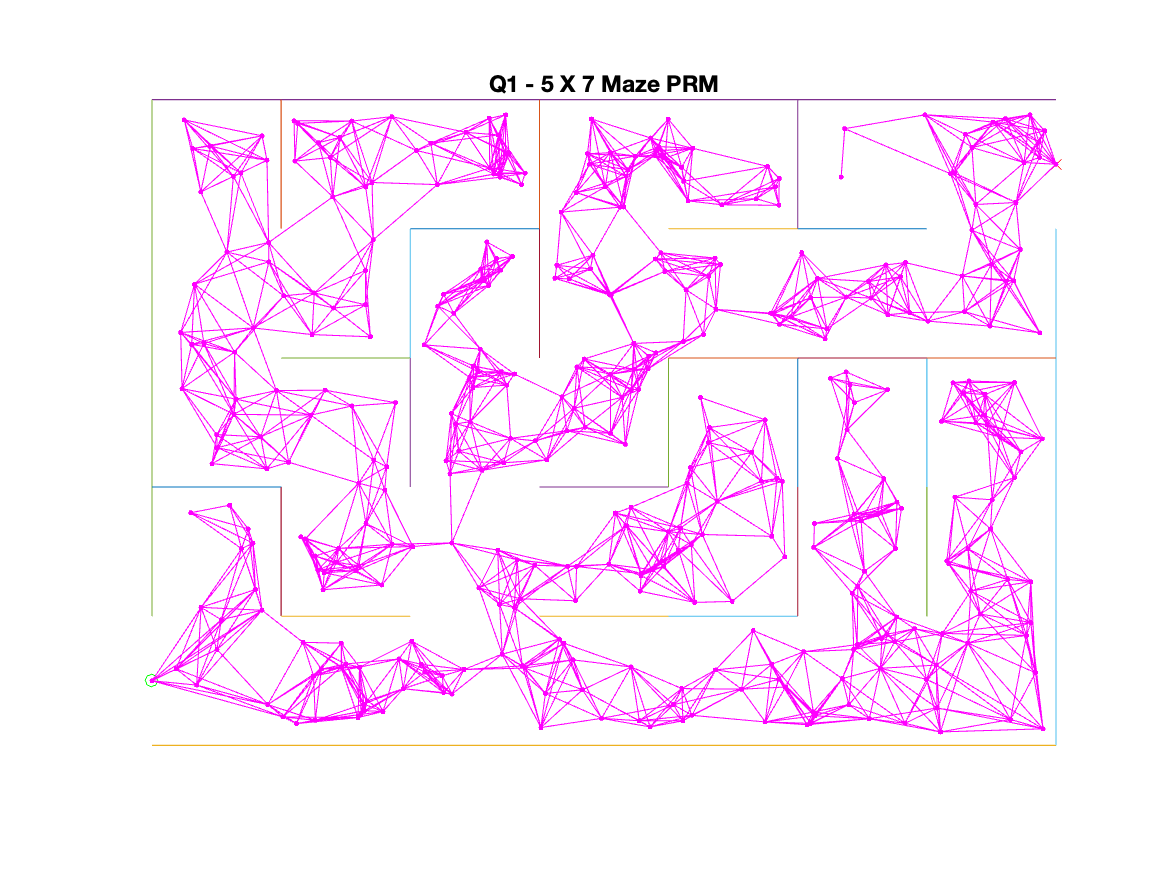
\includegraphics[width=0.8\textwidth]{assignment1_q1.png}
    \caption{PRM graph generation example with k=8}
\end{figure}

\section{Question 2}
The second question involves the implementation of a path planning algorithm to find the shortest path
using the PRM graph generated in the previous question. I chose to implement A* because of its
efficiency and optimality in finding the shortest path. A* involves a cost metric that consists
of a cost-to-come and a heurisitic cost-to-go. I chose to use the Euclidean distance between two
nodes to assign edge costs for computing the cost-to-come. I also chose to use the Manhattan distance
heurisitic for computing the lower bound cost estimate for going from the current node to the goal node.
These metrics are commonly used in path planning algorithm and are efficient to compute for the 2D maze.
The A* implementation involves defining a priority queue to store the nodes to be expanded along with their
cost-to-come and total cost. The algorithm iteratively expands the node with the lowest total cost until
the goal node is reached. When a node that has not been visited before is reached, the cost-to-come and total
cost using the heurisitic are computed and the node is added to the priority queue. If a node that has been visited
before is reached, the cost-to-come is updated if the new cost-to-come is lower than the previous cost-to-come.
This ensures that the algorithm finds the optimal path. When the goal node is reached, any node in the priority queue with a cost-to-come greater than
or equal to the cost-to-come of the goal node is pruned. The final path is then reconstructed by backtracking
from the goal node to the start node. The parent node of each node is stored in a parent array during the search
to facilitate the backtracking procedure. The path is shown below in \textbf{Figure 2}, which took
on average 0.05s to complete.

\begin{figure}[h]
    \centering
    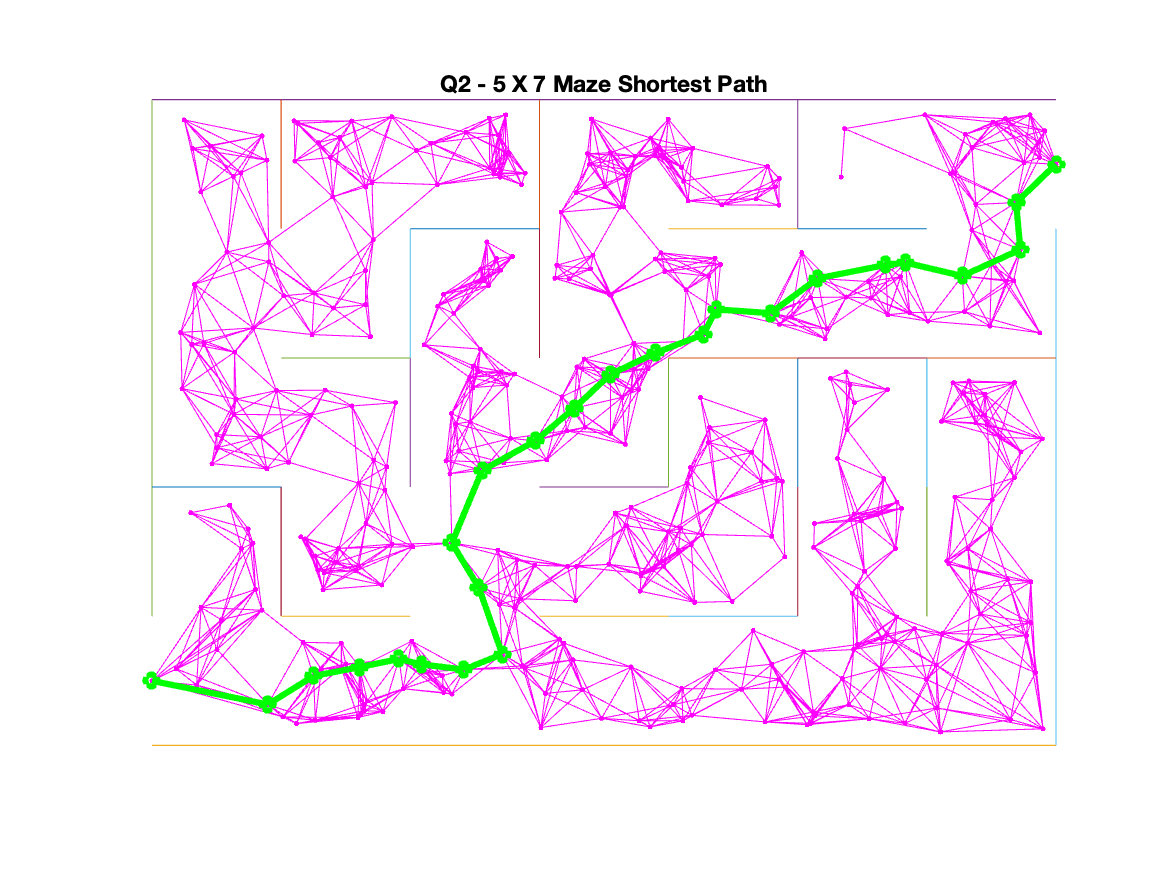
\includegraphics[width=0.8\textwidth]{assignment1_q2.png}
    \caption{A* path planning example}
\end{figure}

\section{Question 3}
The third question involves solving large mazes using an optimized version of the algorithms
implemented so far. I struggled to get 40x40 mazes completed within 20s, even with optimizations
presented in class. In my best attempt, I used a non-uniform Gaussian sampling technique, specifically
bridge sampling as its known to be useful for sampling small corners and narrow passages.
The key idea with this approach is to sample two points within a Gaussian distribution
and save the midpoint of the two points as a milestone if both points are in collision space, thus
allowing for more efficient sampling in narrow passages, which is common in large mazes.
With this, I also implemented a lazy collision checking approach to reduce the number of collision checks
between nodes. This involves only checking for edge collisions when an edge is being considered during the
A* search, rather than during the graph construction process. This is known to provide up to
10x speedups in path planning algorithms, as stated in lecture. Despite these optimizations, I
was only able to complete 25x25 mazes within 9s on average, and 40x40 mazes within 35s. With
25x25 mazes, I found that k=15 and 2500 samples were optimal for consistently finding a path
while also aiming to minimize computational time. However, with 40x40 mazes, I found that k=20
and 6000 samples were required to have about a 75\% success rate in finding a path.
While further optimizations could be made, such as using KD-trees for nearest neighbor searches,
I decided to try a simpler uniform sampling approach where the maze is divided into a grid
and a point is sampled from each grid cell. This approach was able to complete 45x45 mazes
within 20s on average, when using lazy collision checking and k=4 (in this case the number
of samples is based on the size of the maze). An example path is shown below in \textbf{Figure 3}.

\begin{figure}[h!]
    \centering
    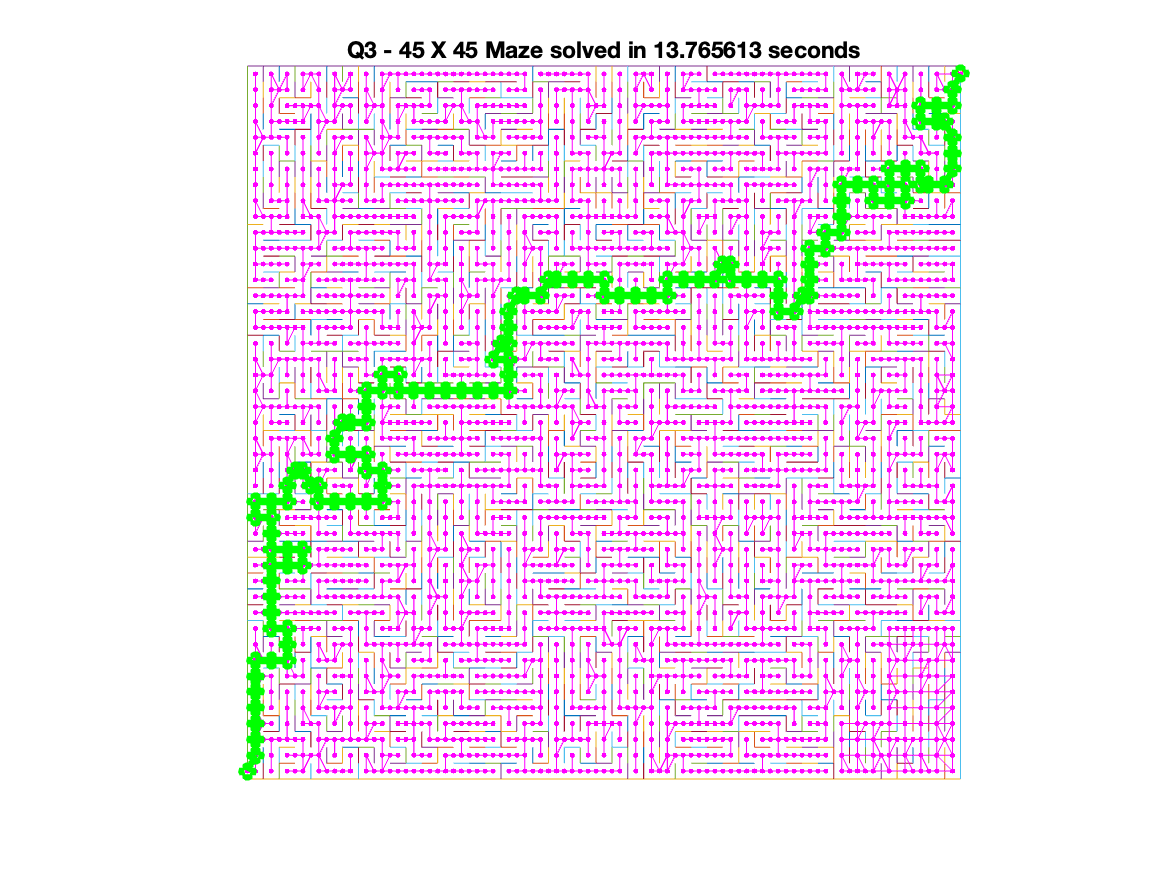
\includegraphics[width=1\textwidth]{assignment1_q3.png}
    \caption{Optimized PRM and A* path planning example}
\end{figure}

Note that since lazy collision checking is used, the plot shows edges that intersect with obstacles.
This is because if an edge is not explored during the A* search, it is not checked for collisions and thus
is not removed from the graph. This can be seen in \textbf{Figure 3} in the top left and bottom right corners,
where there is a higher density of edges resulting from violating edges that were not checked for collisions
as A* did not explore them.

\section{MATLAB Code}

The MATLAB code for these implementations are provided here, as well as are attached in the submission.

\lstinputlisting[
frame=single,
numbers=left,
style=Matlab-editor
]{ROB521_assignment1.m}

\end{document}